%%%%%%%%%%%%%%%%%%%%%%%%%%%%%%%%%%%%%%%%%%%%%%%%%%%%%%%%%%%%
% \begin{frame}{Presentation Structure}
%   \begin{itemize}[<+->]
%     \item Introduction / Quantum Scrambling
%     \item Quantum Circuit Models / Theory
%     \item Results / Entanglement Entropy and OTOC
%     \item Future Directions
%   \end{itemize}
%   \end{frame}
  
  %%%%%%%%%%%%%%%%%%%%%%%%%%%%%%%%%%%%%%%%%%%%%%%%%%%%%%%%%%%%
  \begin{frame}{Introduction}
    \begin{block}<+->{Our Question}
    In an evolving many-body system, how we can describe the dynamics of information within?
    \end{block}
    \begin{block}<+->{A Proposition}
      For sufficiently generic unitary evolution, we expect information to become \textit{scrambled} amongst the degrees of freedom of our system, such that it is inaccessible to local probes.
      \end{block}
    % The set-up of our question is as follows; 
    % Given a many-body system, for example a system of qubits or many particles, 



    %combined notion of operator spreading and growth in entanglement entropy.
    %where does this happen
    % why do we study it?
    %our central question
  

  \end{frame}
\begin{frame}{Introduction}
  \begin{block}{Our Question}
    In an evolving many-body system, how we can describe the dynamics of information within?
  \end{block}
  \begin{block}{A Proposition}
  For sufficiently generic unitary evolution, we expect information to become \textit{scrambled} amongst the degrees of freedom of our system, such that it is inaccessible to local probes.
  \end{block}
  % How can we prove our proposition?
  This process is known as \textbf{Quantum Scrambling}. We aim to investigate this process in many-body quantum systems.  

\end{frame}
  %%%%%%%%%%%%%%%%%%%%%%%%%%%%%%%%%%%%%%%%%%%%%%%%%%%%%%%%%%%%
\begin{frame}{Quantum Scrambling}
  The set-up:
  \begin{itemize}
    \item System with many particles, e.g spin chain or qubit system
    \item Information is encoded as a string of operators e.g $ \mathcal{O} = X\otimes I\otimes Z\otimes Y\otimes I$
    \item System evolves via unitary conjugation $\to$ $\mathcal{O}(t) = U \mathcal{O} U^{\dagger}$
  \end{itemize}
      How can we tell if information has been scrambled? We should observe:
  \begin{columns}
    \vspace{-5cm}
    \begin{column}{0.55\textwidth}
      \vspace{-1.35cm}
      
  \begin{itemize}
    \item An increase in the support of a quantum operator - known as \textit{operator spreading}.
    \begin{itemize}
      \item Local operator: $I I I X_i I I I$
      \item Global operator: $X_1 X_2 X_3 X_4 X_5 X_6 X_7$
    \end{itemize}
    \item A highly entangled system, signified by a growth in \textit{entanglement entropy}
  \end{itemize}
\end{column}
\begin{column}{0.45\textwidth}
    \begin{figure}
      % \vspace{-1.35cm}
      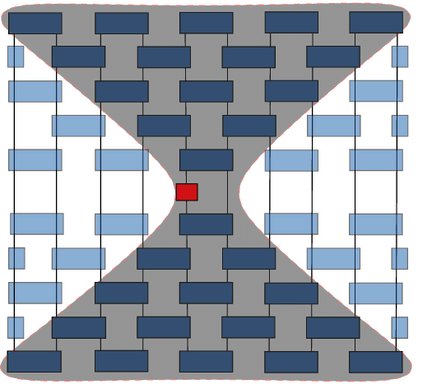
\includegraphics[width=0.6\textwidth]{QS_Images/lightcone.png}
      \caption{Emergent light-cone structure}
    \end{figure}
\end{column}
\end{columns}
  % Operator spreading and Entanglement entropy are key markers. Insert images here

    % Operator spreading and the entanglement entropy are key markers for quantum scrambling and allow us to quantify the phenomenon. We can simulate a quantum system and calculate these. 
\end{frame}

\begin{frame}{Entanglement Entropy}
  \begin{columns}
    \begin{column}{0.45\textwidth}
      \begin{center}
        \underline{Entanglement in state description}
        \begin{figure}
          \vspace{-0.3cm}
          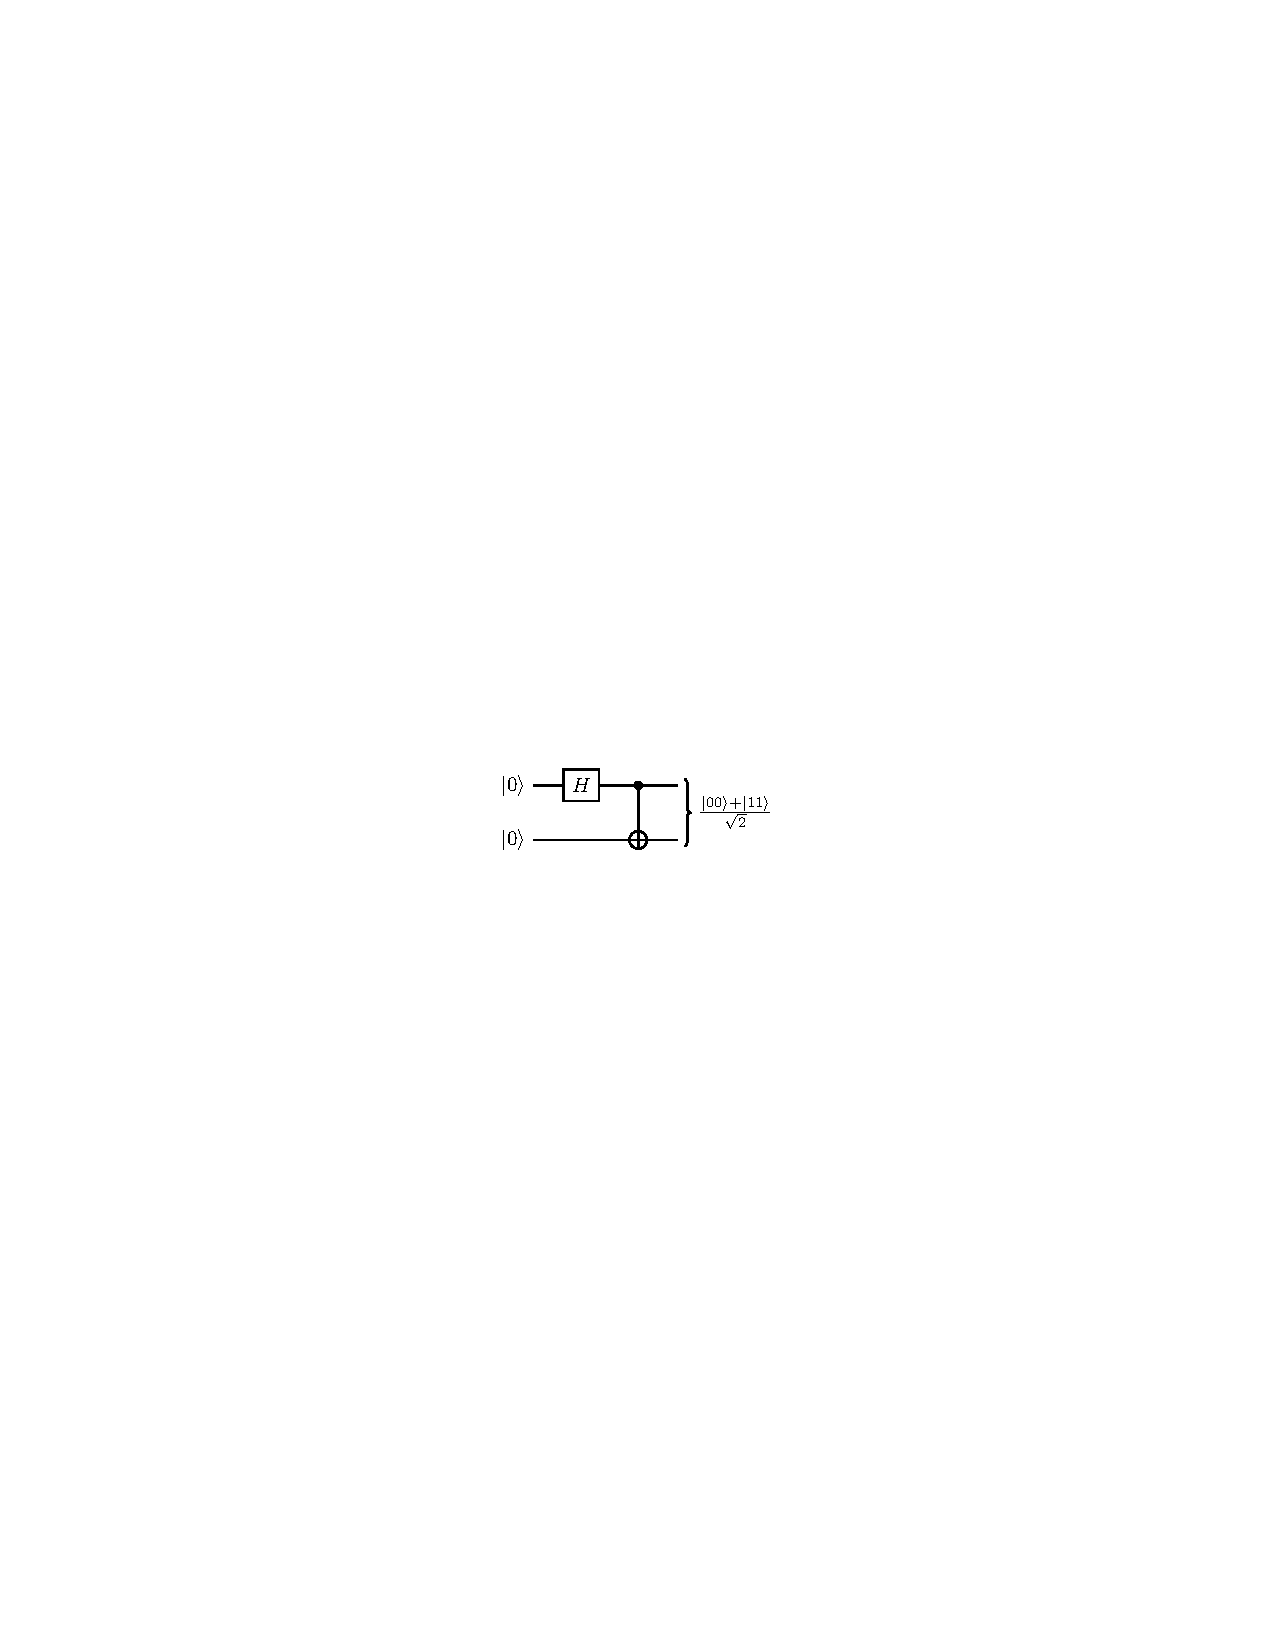
\includegraphics[width = 0.8\textwidth]{QS_Images/BeLL_State.pdf}
        \end{figure}
      \end{center}
    \end{column}


    \begin{column}{0.45\textwidth}
      \begin{center}
        \vspace{-0.45cm}
          \underline{Entanglement in operator space}
          \begin{align*}
            T^{\dagger} X T = \frac{X - Y}{\sqrt{2}}, && T^{\dagger} Y T = \frac{X + Y}{\sqrt{2}}
          \end{align*}
      \end{center}
      
    \end{column}
  \end{columns}

  %In addition to operator spreading, systems that exhibit quantum scrambling show a growth in entanglement entropy. 
  \begin{itemize}
    \item Quantify entanglement using entanglement entropy. 
    \item Initial operator string (e.g a product of Pauli Operators) becomes a product of superpositions of operators $\implies$ entanglement entropy grows
    \item We specifically look at the (bipartite) Von Neumann Entropy, 
    \begin{align*}
      S_A = - \text{tr}(\rho_A\log_2(\rho_A))
    \end{align*}
    Entanglement entropy grows linearly in time, then saturates at the Page value \cite{Page_1993}: $S_{\text{max}} \equiv \text{ln}|A|$.   
  \end{itemize}
  

 

  
\end{frame}
  %change this two breaking it down into consituents, show two pictures, one of operator spreading and entanglement entropy graph, briefly explain both

\begin{frame}{Why?}
  Some motivation:
  \begin{itemize}
    \item Dates back to study of black holes and the black hole information paradox.
    \item Recently seen great attention in condensed matter, quantum information and quantum gravity.
    \item Lack of understanding of evolution in quantum chaotic systems.
    \item Reveals an irreversibilty of generic unitary dynamics - can no longer recover information with local probes.
    \item Proposed to characterise dynamics in ultra-cold atom systems.
  \end{itemize}

  Now back to our proposition...
\end{frame}

  \begin{frame}{Simulating a Quantum System}
    \begin{block}<+->{A Proposition}
      For sufficiently generic unitary evolution, we expect information to become \textit{scrambled} amongst the degrees of freedom of our system. 
      \end{block}
\begin{columns}

\begin{column}{0.5\textwidth}
  \vspace{-0.8cm}

      To prove this proposition, we simulate our system as a quantum circuit. More specifically, we utilise two circuit models:
      \begin{itemize}
        \item Clifford circuits.
        \item Non-interacting Fermion circuits.
      \end{itemize}
      Both models are classically simulable, such that they can be simulated with polynomial effort. 
  
\end{column}

\begin{column}{0.475\textwidth}
  \vspace{-2cm}
  \begin{figure}
    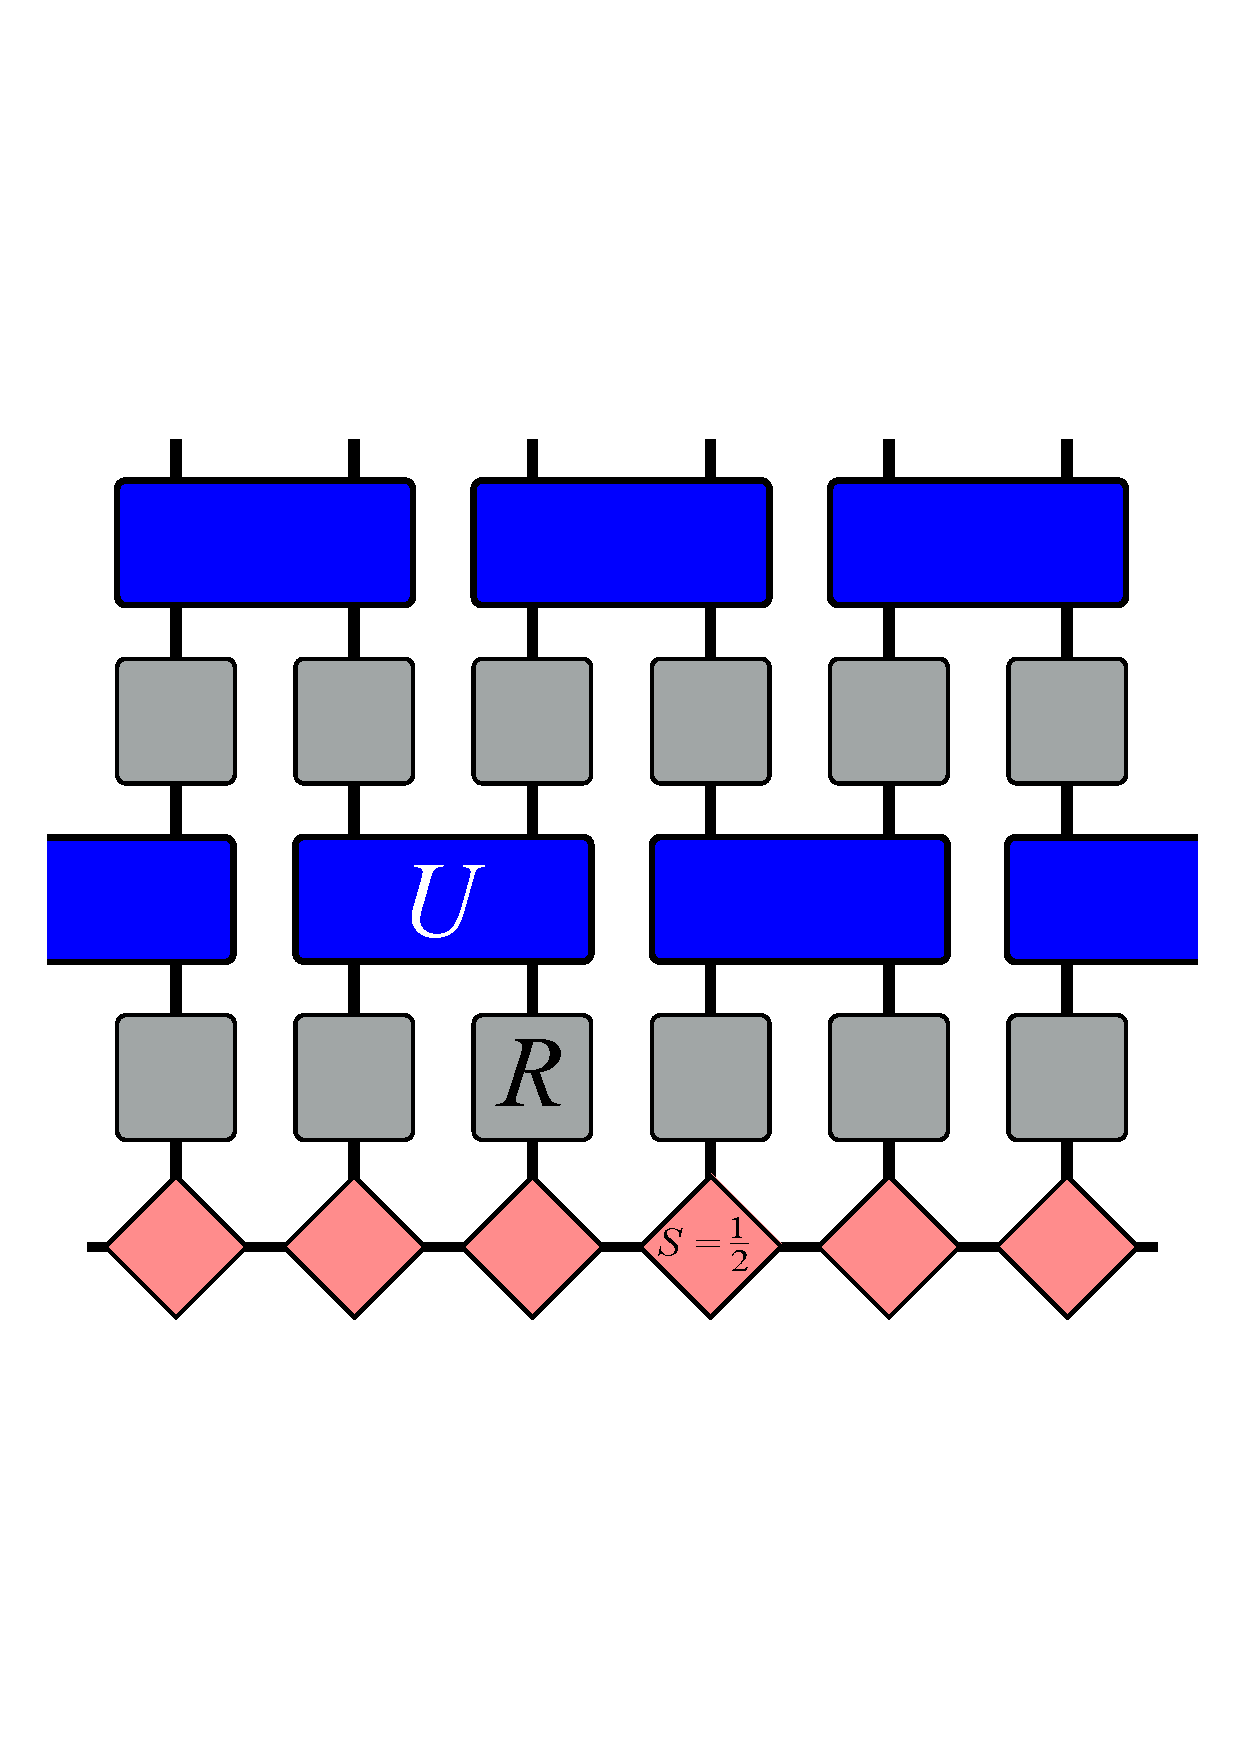
\includegraphics[width = 0.8\textwidth]{QS_Images/quantum circuit.pdf}
    \vspace{-2cm}
    \caption{'Brickwork' quantum circuit \cite{Nahum_2017}}
  \end{figure}
\end{column}
  
\end{columns}

\end{frame}
